\section{Introducción Teórica}

\subsection{El Problema y su representación}

El problema comienza con un horno industrial cilíndrico utilizado para fundir metales. Dicho horno tiene una pared interior y una exterior, cuyas temperaturas (la de las paredes) son conocidas en determinados puntos. Sabemos que la pared exterior tiene un límite de temperatura máxima, y nuestro objetivo es determinar si dicha temperatura máxima es alcanzada o no. Para ello, buscamos los puntos en el horno cuya temperatura alcance los 500 grados celcius. Si esta temperatura es cercana al borde exterior se corre peligro por parte de los trabajadores de una hipotética fábrica que utilice dicho horno.\\


\begin{wrapfigure}{r}{0.5\textwidth}
  \vspace{-20pt}
  \begin{center}
    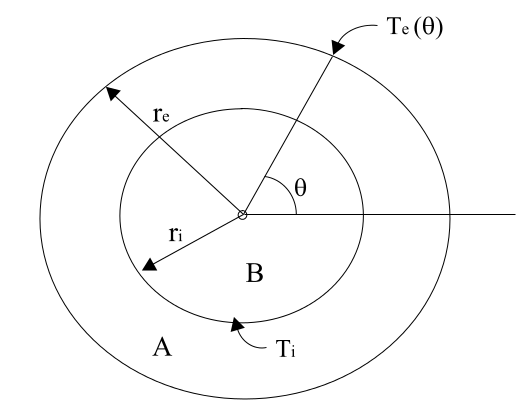
\includegraphics[scale= 0.4]{../Horno.png}
  \end{center}
  \vspace{-20pt}
  \caption{Corte del horno}
  \vspace{-10pt}
  \label{fig:corteHorno}
\end{wrapfigure}


Una instancia del problema equivale a un corte del horno como se ilustra en la figura ~\ref{fig:corteHorno}. Dado que la medición de temperatura en el horno puede realizarse en infinitos puntos, discretizamos el problema fijando la ubicación de los mismos de la siguiente manera; Dividimos el horno en \textbf{\textit{n}} cantidad de ángulos de tamaño $\Delta_{\theta}$ y en \textbf{\textit{m}} cantidad de radios, de tamaño $\Delta_{r}$. Analizaremos las temperaturas en los puntos donde se unen las divisiones entre ángulos y radios. Recordemos que los puntos de la pared interna y externa son dato.\\
\\

La temperatura en un punto $t_{(j,k)}$, con $j \in [0, m]$ y $k \in (0, n]$ estará determinado por la ecuación de Laplace descripta a continuación:

%TODO : estos limites estan bien?? para j y k arriba..?

$$ \frac{\partial^{2}T(r,\theta)}{\partial r^{2}} + \frac{1}{r} \frac{\partial T(r,\theta)}{\partial r} + \frac{1}{r^{2}} \frac{\partial^{2}T(r,\theta)}{\partial \theta^{2}} = 0$$\\

Sin embargo utilizaremos una aproximación de esta función que depende de los cuatro puntos que rodean a $t_{(j,k)}$:


$$ \frac{t_{(j-1,k)} - 2t_{(j,k)} + t_{(j+1,k)}}{\Delta_{r} ^{2}} + \frac{1}{r} \frac{t_{(j,k)} - t_{(j-1,k)}}{\Delta_{r}} + \frac{1}{r^{2}} \frac{t_{(j,k-1)} - 2t_{(j,k)} + t_{(j,k+1)}}{\Delta_{\theta} ^{2}} = 0$$

Despejamos las incógnitas $t_{(j,k)}$, $t_{(j+1,k)}$, $t_{(j-1,k)}$, $t_{(j,k+1)}$ y $t_{(j,k-1)}$ para obtener una ecuación (un sistema de ecuaciones) que dependa de ellas. Resulta la siguiente fórmula:

%TODO: Deberia desarrollarla????? Pajaaaaaa, pero si hay que ocupar lugar, lo hago.

$$  t_{(j,k)} (-\frac{2}{\Delta^2_r}+\frac{1}{r \Delta_r}-\frac{2}{r^2 \Delta^2_\theta}) + t_{(j+1,k)} (\frac{1}{\Delta^2_r}) + t_{(j-1,k)} (\frac{1}{\Delta^2_r}-\frac{1}{r \Delta_r}) + t_{(j,k+1)} (\frac{1}{r^2 \Delta^2_\theta}) + t_{(j,k-1)} (\frac{1}{r^2 \Delta^2_\theta}) = 0$$ \\


Una vez planteadas estas ecuaciones para cada $ṭ_{(j,k)}$, resolvemos que el sistema $Ax = b$ estará formado por $n*m$ ecuaciones con la misma cantidad de incógnitas. El valor lo justificamos debido a la cantidad de combinaciones entre los índices j y k (cantidad de ángulos por cantidad de radios). Otra forma de razonar este resultado es pensando que en cada anillo generado por la partición del horno en \textbf{\textit{m}} radios, habrá \textbf{\textit{n}} incógnitas generadas a su vez por la particion en ángulos. \\
Esta cantidad incluye los valores $t_{(0,k)}$ y $t_{(n-1,k)}$ (los valores de temperatura en la pared interior y exterior respectivamente), por lo que en sus ecuaciones habrá un único coeficiente con valor 1 en la posición que corresponde a estas incógnitas y su valor b será el que se pase por parámetro. Para el resto de los $t_{(j,k)}$ los coeficientes corresponderan a los coeficientes descriptos en la ecuación de arriba, y su b será cero, también respetando dicha ecuación.


\subsection{Solucionando el problema}

Dadas las herramientas aprendidas en la materia (sistemas de ecuaciones lineales, y sus métodos de solución, como Eliminación Gaussiana o factorización LU) queremos representar las temperaturas como incógnitas de un sistema lineal de ecuaciones. Una vez logrado este objetivo (explicado en la sección anterior) utilizamos dichas herramientas.

\subsubsection{Eliminación Gaussiana}
Dada una matriz A $\in R^{nxn}$ queremos resolver el sistema $Ax = b$. El algoritmo de Eliminación Gaussiana se usa para simplificar el sistema de ecuaciones ya que produce una matriz triangular superior equivalente a la original. Esto facilita el despeje de las incógnitas con el uso de otro algoritmo llamado Backward Substitution. Las tres operaciones principales que se llevan a cabo son, suma entre filas, multiplicación de una fila por un coeficiente distinto de cero e intercambio de filas. Dichas operaciones mantienen la equivalencia.

%TODO: puedo hablar aca de los detalles de implementacion?? o va en desarrollo??

El método Backward Substitution consiste en la obtención de los valores de las incógnitas a partir de la matriz triangulada. El método recorre cada fila de esta matriz en orden decreciente en filas. Con lo que el despeje de las incógnitas simplemente consiste en despejar el valor de la diagonal respecto al resto de los valores ya obtenidos en iteraciones anteriores.

El algoritmo de Factorización LU surge ante el problema que se presenta cuando queremos resolver un sistema de ecuaciones similar a uno anteriormente resuelto. Dado el sistema de ecuaciones $Ax = b$, una vez obtenida la matriz triangulada, no queda registro alguno de las operaciones realizadas. Si estas fueran guardadas de alguna manera, podríamos reflejarlas en $b^{*}$  para cada nuevo sistema $Ax = b^{*}$. Repetir E.G. tendría un costo adicional de $O(n^{3})$ tiene como fin evitar hacer cuentas de mas, reduce la repeticion de cuentas de complejidad $O(n^{3})$ .

diagonal dominante


